% \documentclass{report}
% \usepackage[utf8]{inputenc}
\usepackage[spanish,english]{babel}
\usepackage{graphicx}
\usepackage{amsmath}
\usepackage[left=2cm,right=2cm,bottom=2cm,top=2cm]{geometry}
\usepackage{amssymb}
\usepackage{hyperref}
\hypersetup{
	colorlinks=true,
	linkcolor=blue,
	filecolor=magenta,
	urlcolor=blue,
}
\usepackage{mathrsfs}
\usepackage{amsfonts}
\usepackage{amsthm}
\usepackage{bbold}
\usepackage{physics}
\usepackage{siunitx}
\usepackage{cancel}
\usepackage{caption}
\usepackage{subcaption}
\usepackage{multicol}
\usepackage{color}
\usepackage{pdfpages}
\usepackage{empheq}
\usepackage{feynmf}
\usepackage{tikz}
\usepackage{titlesec}
\usepackage{mathtools}

\decimalpoint

\setlength{\columnseprule}{.5pt}
\def\columnseprulecolor{\color{black}}

\graphicspath{{images/}}

\usepackage{setspace}
\usepackage{gensymb}
% \usepackage{mathpazo}
\usepackage{authblk}
\usepackage{fancyhdr}


\newcommand{\thedate}{February 3, 2025}
\newcommand{\HW}{1}
\newcommand{\kcoulomb}{\frac{1}{4\pi\epsilon_0}}

\usepackage{mathptmx}
% Math fonts need to be loaded before fontspec

% \usepackage{fontspec}
% \usepackage{times}
% \setmainfont{Times New Roman}
% \setmainfont{Tex Gyre Termes}
% \setmainfont{TeXGyreTermes}
% \usepackage{palatino}




\documentclass[aspectratio=1610]{beamer}
\usepackage[utf8]{inputenc}
\usepackage{amsmath}
\usepackage{amsfonts}
\usepackage{amssymb}
\usepackage{bbold}
\usepackage{graphicx,fancybox}
\usepackage{babel}
\usepackage{minted}
\usepackage{wrapfig}
\usepackage{verbatim}
\usepackage{appendixnumberbeamer}
\usepackage{multicol}
\usepackage{physics}
\usepackage{hyperref}
\hypersetup{
	colorlinks=true,
	linkcolor=blue,
	filecolor=magenta,
	urlcolor=blue,
}

\setlength{\columnseprule}{.5pt}
\def\columnseprulecolor{\color{black}}


\graphicspath{{Images/}}

\setbeamertemplate{footline}[frame number]
\beamertemplatenavigationsymbolsempty
% \usetheme{Madrid}
\usetheme{Warsaw}

\addtobeamertemplate{footline}{\hypersetup{allcolors=.}}{}
% \definecolor{uprmgreen}{RGB}{51, 113, 55}
\definecolor{crimsonflame}{RGB}{158, 27, 50}
\usecolortheme[named=crimsonflame]{structure}

\usefonttheme{professionalfonts}
\usepackage{mathptmx}
% \renewcommand\familydefault{\rmdefault}

\newcommand{\thedate}{\today}
\newcommand{\HW}{1}
\newcommand{\kcoulomb}{\frac{1}{4\pi\epsilon_0}}


% \useoutertheme{split}
% \title{Template}
\title[Qual Review]{Qualifier Review\\ Quantum Mechanics}
\date{\thedate}

%%%%%%%%%%%%%%%
% for documents
% \author{Guillermo Fidalgo Rodríguez} %[1] is to indicate connection with affil institute
% \author{Tetiana}
% \author{Roy}
% \affil[1]{University of Puerto Rico - Mayagüez, Physics Department}

%%%%%%%%%%%%%%%
% for beamer
\author[G. Fidalgo]{Guillermo A. Fidalgo Rodríguez}
\institute[UA]{University of Alabama}
% \logo{
\includegraphics[width = 1in]{uprm_logo.png}}
% \logo{
\includegraphics[width = 1cm]{UA_logo.jpg}}
%%%%%%%%%%%%%%%


\begin{document}

%%%%%%%%%%%%%%%%%%% For Articles or reports
% \maketitle
% Set the page style to "fancy"...
% \pagestyle{fancy}
%... then configure it.
% \fancyhead{} % clear all header fields
% \fancyhead[L]{\textbf{Guillermo Fidalgo} }
% \fancyhead[C]{Homework \HW}
% \fancyhead[R]{\thedate}
% \fancyfoot{} % clear all footer fields
% \fancyfoot[LE,RO]{\thepage}
% \fancyfoot[LO,CE]{From: K. Grant}
% \fancyfoot[CO,RE]{To: Dean A. Smith}
% Some content:
% My content
% \begin{enumerate}
% 	
\section[Wave Functions]{Wave Functions; State Functions and operators; uncertainty principle}
\subsection{Wave Functions}

\begin{frame}{Wave Functions}
The Schrödinger equation describes how the quantum state of a physical system changes over time. The wave function, denoted by $\Psi$, is a complex-valued function that contains all the information about the system.

\begin{block}{Schrödinger Equation}
    \begin{equation*}
        i\hbar \frac{\partial \Psi(\mathbf{r}, t)}{\partial t} = \hat{H} \Psi(\mathbf{r}, t)
    \end{equation*}
    where $\hat{H}$ is the Hamiltonian operator, which represents the total energy of the system.

    In one dimension, the time-dependent Schrödinger equation can be written as:
    \begin{equation*}
        % -\frac{\hbar^2}{2m} \frac{d^2 \Psi(x)}{dx^2} + V(x) \Psi(x) = E \Psi(x)
        i\hbar \frac{\partial \Psi(x, t)}{\partial t} = -\frac{\hbar^2}{2m} \frac{d^2 \Psi(x, t)}{dx^2} + V(x) \Psi(x, t)
    \end{equation*}
    where $V(x)$ is the potential energy and $m$ is the mass of the particle.

\end{block}

\end{frame}

\begin{frame}{Wave Functions (cont)}
The wave function collapses when a measurement (i.e. observation) is made.
In QM, we may only measure the probability of observing the position of a particle at specific time $t$ by computing $|\Psi(x,t)|^2$ or more precisely
\begin{block}

    \[
        \int_a^b |\Psi(x,t)|^2 \dd{x} = \int_a^b \Psi^*(x,t) \Psi(x,t) \dd{x}
    \]

\end{block}
\end{frame}

\subsection{Stats review}

\begin{frame}
    \frametitle{Some important stats review}
\begin{description}
    \item[mean] is the numerical average of multiple measurements at a time.
    \item[median] the 50th percentile, second quantile, i.e. the value at which there
    is the same probability to measure any value below or after this value.
    \item[mpv] the number that has the highest probability to be measured.
    Another name for the ``mode''.
    \item[expectation value]  this a little misnomer. Same as the mean value in our case.
\end{description}
We comput these as follows


\begin{onlyenv}<1>

    \begin{block}{mean/expectation value}
        The average is computed for a number of different moments of j as follows
        \begin{gather}
            \ev{j}= \sum_{j=0}^\infty j P(j) \qq{;} \ev{j^2} = \sum_{j=0}^\infty j^2 P(j) \qq{\dots} \ev{j^n} = \sum_{j=0}^\infty j^n P(j)\\
           \text{In General} \hspace{1cm} \boxed{\ev{f(j)} = \sum_{j=0}^\infty f(j) P(j)}
        \end{gather}

    \end{block}

\end{onlyenv}

\begin{onlyenv}<2>

    \begin{block}{median}
        The formula depends on the number of observations or data points. First we order the data list
        $\{X_1, X_2, \dots, X_n\}$ then
        \[
        \text{Median} =
        \begin{cases}
            \frac{X_{n/2} + X_{(n/2)+1}}{2} & \text{if } n \text{ is even} \\
            X_{(n+1)/2} & \text{if } n \text{ is odd}
        \end{cases}
        \]

    \end{block}

\end{onlyenv}

\end{frame}


\begin{frame}{Variance and Standard Deviation}
    These measure the spread of a distribution (particularly the standard deviation).
    First we find the deviation of each value from the mean.
    \[
        \Delta j = j - \ev j
    \]

    then we find the average of the \textit{square} of the deviations (why? Because the average deviation is \textbf{always} zero!). So now
    \begin{align*}
        \sigma^2 & =\ev{(\Delta j)^2} = \sum(\Delta j)^2 P(j)=\sum(j-\ev{j})^2 P(j) \\
        & =\sum\left(j^2-2 j \ev{j} + \ev{j}^2\right) P(j) \\
        & =\sum j^2 P(j)-2 \ev{j} \sum j P(j)+\ev{j}^2 \sum P(j) \\
        & =\ev{ j^2}-2\ev{ j}\ev{ j}+\ev{ j}^2=\ev{ j^2}-\ev{ j}^2 .
    \end{align*}

    Finally $$\sigma = \sqrt{\ev{ j^2}-\ev{ j}^2}$$
\end{frame}


\begin{frame}
    \frametitle{Probability density and properties for continuous functions}
    $$ P_{ab} = \int_a^b \rho(x) \dd{x}$$
    is the probability that $x$ lies between $a$ and $b$. The other properties are:
    \begin{gather}
    \int_{-\infty}^{+\infty} \rho(x) d x=1 \\
    \langle x\rangle=\int_{-\infty}^{+\infty} x \rho(x) d x \\
    \langle f(x)\rangle=\int_{-\infty}^{+\infty} f(x) \rho(x) d x \\
    \sigma^2 \equiv\left\langle(\Delta x)^2\right\rangle=\left\langle x^2\right\rangle-\langle x\rangle^2
\end{gather}

\end{frame}

\subsection{Back to the wave function}


% \subsection{State Functions and operators}
% \begin{frame}{State Functions and operators}

% \end{frame}



% \subsection{Uncertainty Principle}
% \begin{frame}{Uncertainty Principle}

% \end{frame}

% \begin{frame}{Uncertainty Principle}
% 	\begin{block}{Heisenberg's Uncertainty Principle}
% 		\begin{equation*}
% 			\Delta x \Delta p \geq \frac{\hbar}{2}
% 		\end{equation*}
% 		where $\Delta x$ is the uncertainty in position and $\Delta p$ is the uncertainty in momentum.
% 	\end{block}
% \end{frame}

% 	% \section{Schrödinger Equation}

% \subsection{Time Dependent Schrödinger Equation}
% \frame{Time Dependent Schrödinger Equation}


% \subsection{Time Independent Schrödinger Equation}
% \frame{Time Independent Schrödinger Equation}

% 	%\section[Potentials]{Exactly Solvable Potentials}

\subsection[Infinite Well]{The Infinite Square Well}

\begin{frame}{The Infinite Square Well}
	Here the potential is of the form
	\[
		V(x) = \begin{cases}
			0      & 0 \leq x \leq a  \\
			\infty & \text{otherwise}
		\end{cases}
	\]
	And as a consequence the Schrödinger equation looks like
	\begin{align*}
		-\frac{\hbar^2}{2m} \dv[2]{\psi}{x} = E \psi &  & \dv[2]{\psi}{x} = -\frac{2mE}{\hbar^2 } \psi    \\
		\dv[2]{\psi}{x} -k^2 \psi                    &  & \text{where } k \equiv \frac{\sqrt{2mE}}{\hbar}
	\end{align*}
	Because $E$ must be at least greater than the smallest $V(x)$, $E\ge 0$ and the solution is of the form
	$$ \psi(x) = A \sin kx + B \cos kx$$

	Now we apply boundary conditions  like $\psi(0) = \psi(a) = 0$ and $\psi(x)$ is continuous. We find that $B = 0$ and
	$$ \boxed{k = k_n = \frac{n \pi}{a} \to E_n = \frac{\hbar^2 k_n^2}{2m} = \frac{\hbar^2 n^2 \pi^2}{2ma^2}} $$

\end{frame}

\begin{frame}
	Now we must find $A$ via the normalization condition.
	$$ \int_0^a |A|^2 \sin[2](kx) \dd{x} = |A|^2 \frac a2 = 1 \qq{so} |A|^2 = \frac 2a$$ We pick the positive real value of $A$ and have that
	$$ \psi_n(x) = \sqrt{\frac{2}{a}} \sin(\frac{n \pi}{a}x)$$
	The lowest energy state is $\psi_1$, called the ground state. The next is $\psi_2$ and so on. Each has energy that is $E_n \propto n^2$ and as a collection, the functions $\psi_n(x)$ have the following properties.

\end{frame}

\begin{frame}{Some notes on $\psi_n(x)$}
	\begin{enumerate}
		\item They are alternately even and odd, with respect to the center of the well: $\psi_1$ is even, $\psi_2$  is odd, $\psi_3$ is even,and so on. True when $V(x)$ is a symmetric function.
		\item As you go up in energy, each state has more nodes according to the figure below(edges don't count). This is universal.
		\item They are mutually orthogonal i.e. $\displaystyle \int \psi_m(x)^* \psi_n(x) \dd x = 0, (m \neq n)$. And in general $$\int \psi_m(x)^* \psi_n(x) \dd{x} = \delta_{mn}$$
	\end{enumerate}

	\begin{figure}
		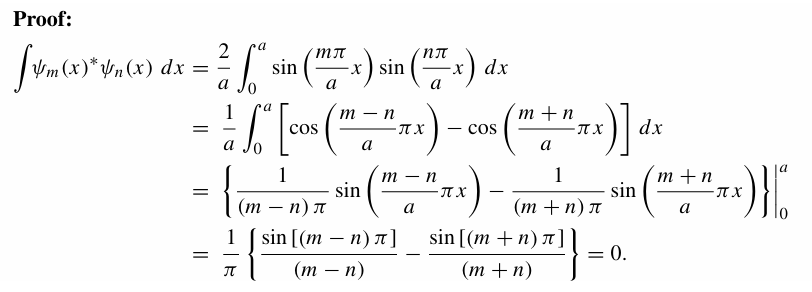
\includegraphics[width = .9\linewidth,trim=0cm 0 0 4mm]{QM_proof1.png}
	\end{figure}

\end{frame}

\begin{frame}{More notes}
	\begin{enumerate}
		\setcounter{enumi}{3}
		\item They are \textbf{complete} i.e. any function can be expressed in terms of linear combinations of $\psi_n(x)$. (This is practically always true but not in general...) $$ f(x) = \sum_{n=1}^{\infty} c_n \psi_n(x)	= \sqrt{\frac 2a } \sum_{n=1}^{\infty} c_n \sin(\frac{n\pi}{a} x)$$ (sometimes called the Dirichlet Theorem). Using Fourier's trick we can get the coefficient $c_n$ to be  $$ c_n = \int \psi_n(x)^* f(x) \dd{x} $$
	\end{enumerate}
\end{frame}

\begin{frame}{Back to the square well}
	The stationary states for the square well are
	\[
		\Psi_n(x,t) = \sqrt{\frac 2a} \sin(\frac{n\pi}{a}x) \exp(-i \frac{n^2\pi^2 \hbar^2}{2ma^2}t)
	\]
	(remember the time factor from eq. \ref{eq:GeneralSol}) and therefore the general solution for the infinite square well is
	\begin{equation}
		\label{eq:sol_sqwell}
		\Psi(x,t) = \sum_{n=1}^{\infty}c_n \sqrt{\frac 2a} \sin(\frac{n\pi}{a}x)e^{-i (n^2\pi^2 \hbar^2/2ma^2)t}
	\end{equation}
	With the $c_n$ to be
	\begin{equation}
		c_n = \sqrt{\frac 2a} \int_{0}^{a} \sin(\frac{n\pi}{a}x) \Psi(x,0) \dd{x}
	\end{equation}

\end{frame}

\subsection{Harmonic Oscillator}
\begin{frame}{The Harmonic Oscillator}
	The potential has the form $$ V(x) = \frac 12 kx^2 = \frac 12 m\omega^2 x^2$$ giving us the following TISE
	$$-\frac{\hbar^2}{2m} \dv[2]{\psi}{x} + \frac 12 m\omega^2x^2 \psi = E \psi$$
	This can be solved in 2 ways : Algebraic (using ladder operators) and Analytic  (power series solution).
	First the Algebraic method
\end{frame}
\begin{frame}{Algebraic method (Ladder operators)}
	We rewrite the TISE in the following form
	\[
		\frac{1}{2m} \qty[\hat{p}^2 + (m\omega x)^2]\psi =E\psi
	\]
	and invoke the ladder operators (I write it here in two equivalent forms Griffiths' and Sakurai's)

	\textbf{Note} $a_+ = a^\dag$ so $a_- = a$ in Sakurai's notation


	\begin{align*}
		\hat{a}_{\pm} = \frac{1}{\sqrt{2\hbar m \omega }} (m\omega x \; \mp i \hat p) &  & \hat{a}_{\pm} = \sqrt{\frac{m\omega}{2\hbar}} \qty(x \mp \frac{i p }{m\omega})
	\end{align*}

\end{frame}

% 	%\include{Questions/P4}
% 	%\include{Questions/P5}
% 	% \include{Questions/P6}
% \end{enumerate}

%%%%%%%%%%%%%%%%%% For Beamer
\begin{frame}
	\titlepage
	\hfill
	
\includegraphics[width=.5in]{Images/UA_logo.jpg}
\end{frame}

\begin{frame}{TOC}
	\tableofcontents
\end{frame}


\section[Wave Functions]{Wave Functions; State Functions and operators; uncertainty principle}
\subsection{Wave Functions}

\begin{frame}{Wave Functions}
The Schrödinger equation describes how the quantum state of a physical system changes over time. The wave function, denoted by $\Psi$, is a complex-valued function that contains all the information about the system.

\begin{block}{Schrödinger Equation}
    \begin{equation*}
        i\hbar \frac{\partial \Psi(\mathbf{r}, t)}{\partial t} = \hat{H} \Psi(\mathbf{r}, t)
    \end{equation*}
    where $\hat{H}$ is the Hamiltonian operator, which represents the total energy of the system.

    In one dimension, the time-dependent Schrödinger equation can be written as:
    \begin{equation*}
        % -\frac{\hbar^2}{2m} \frac{d^2 \Psi(x)}{dx^2} + V(x) \Psi(x) = E \Psi(x)
        i\hbar \frac{\partial \Psi(x, t)}{\partial t} = -\frac{\hbar^2}{2m} \frac{d^2 \Psi(x, t)}{dx^2} + V(x) \Psi(x, t)
    \end{equation*}
    where $V(x)$ is the potential energy and $m$ is the mass of the particle.

\end{block}

\end{frame}

\begin{frame}{Wave Functions (cont)}
The wave function collapses when a measurement (i.e. observation) is made.
In QM, we may only measure the probability of observing the position of a particle at specific time $t$ by computing $|\Psi(x,t)|^2$ or more precisely
\begin{block}

    \[
        \int_a^b |\Psi(x,t)|^2 \dd{x} = \int_a^b \Psi^*(x,t) \Psi(x,t) \dd{x}
    \]

\end{block}
\end{frame}

\subsection{Stats review}

\begin{frame}
    \frametitle{Some important stats review}
\begin{description}
    \item[mean] is the numerical average of multiple measurements at a time.
    \item[median] the 50th percentile, second quantile, i.e. the value at which there
    is the same probability to measure any value below or after this value.
    \item[mpv] the number that has the highest probability to be measured.
    Another name for the ``mode''.
    \item[expectation value]  this a little misnomer. Same as the mean value in our case.
\end{description}
We comput these as follows


\begin{onlyenv}<1>

    \begin{block}{mean/expectation value}
        The average is computed for a number of different moments of j as follows
        \begin{gather}
            \ev{j}= \sum_{j=0}^\infty j P(j) \qq{;} \ev{j^2} = \sum_{j=0}^\infty j^2 P(j) \qq{\dots} \ev{j^n} = \sum_{j=0}^\infty j^n P(j)\\
           \text{In General} \hspace{1cm} \boxed{\ev{f(j)} = \sum_{j=0}^\infty f(j) P(j)}
        \end{gather}

    \end{block}

\end{onlyenv}

\begin{onlyenv}<2>

    \begin{block}{median}
        The formula depends on the number of observations or data points. First we order the data list
        $\{X_1, X_2, \dots, X_n\}$ then
        \[
        \text{Median} =
        \begin{cases}
            \frac{X_{n/2} + X_{(n/2)+1}}{2} & \text{if } n \text{ is even} \\
            X_{(n+1)/2} & \text{if } n \text{ is odd}
        \end{cases}
        \]

    \end{block}

\end{onlyenv}

\end{frame}


\begin{frame}{Variance and Standard Deviation}
    These measure the spread of a distribution (particularly the standard deviation).
    First we find the deviation of each value from the mean.
    \[
        \Delta j = j - \ev j
    \]

    then we find the average of the \textit{square} of the deviations (why? Because the average deviation is \textbf{always} zero!). So now
    \begin{align*}
        \sigma^2 & =\ev{(\Delta j)^2} = \sum(\Delta j)^2 P(j)=\sum(j-\ev{j})^2 P(j) \\
        & =\sum\left(j^2-2 j \ev{j} + \ev{j}^2\right) P(j) \\
        & =\sum j^2 P(j)-2 \ev{j} \sum j P(j)+\ev{j}^2 \sum P(j) \\
        & =\ev{ j^2}-2\ev{ j}\ev{ j}+\ev{ j}^2=\ev{ j^2}-\ev{ j}^2 .
    \end{align*}

    Finally $$\sigma = \sqrt{\ev{ j^2}-\ev{ j}^2}$$
\end{frame}


\begin{frame}
    \frametitle{Probability density and properties for continuous functions}
    $$ P_{ab} = \int_a^b \rho(x) \dd{x}$$
    is the probability that $x$ lies between $a$ and $b$. The other properties are:
    \begin{gather}
    \int_{-\infty}^{+\infty} \rho(x) d x=1 \\
    \langle x\rangle=\int_{-\infty}^{+\infty} x \rho(x) d x \\
    \langle f(x)\rangle=\int_{-\infty}^{+\infty} f(x) \rho(x) d x \\
    \sigma^2 \equiv\left\langle(\Delta x)^2\right\rangle=\left\langle x^2\right\rangle-\langle x\rangle^2
\end{gather}

\end{frame}

\subsection{Back to the wave function}


% \subsection{State Functions and operators}
% \begin{frame}{State Functions and operators}

% \end{frame}



% \subsection{Uncertainty Principle}
% \begin{frame}{Uncertainty Principle}

% \end{frame}

% \begin{frame}{Uncertainty Principle}
% 	\begin{block}{Heisenberg's Uncertainty Principle}
% 		\begin{equation*}
% 			\Delta x \Delta p \geq \frac{\hbar}{2}
% 		\end{equation*}
% 		where $\Delta x$ is the uncertainty in position and $\Delta p$ is the uncertainty in momentum.
% 	\end{block}
% \end{frame}


% % \section{Schrödinger Equation}

% \subsection{Time Dependent Schrödinger Equation}
% \frame{Time Dependent Schrödinger Equation}


% \subsection{Time Independent Schrödinger Equation}
% \frame{Time Independent Schrödinger Equation}

% \section[Potentials]{Exactly Solvable Potentials}

\subsection[Infinite Well]{The Infinite Square Well}

\begin{frame}{The Infinite Square Well}
	Here the potential is of the form
	\[
		V(x) = \begin{cases}
			0      & 0 \leq x \leq a  \\
			\infty & \text{otherwise}
		\end{cases}
	\]
	And as a consequence the Schrödinger equation looks like
	\begin{align*}
		-\frac{\hbar^2}{2m} \dv[2]{\psi}{x} = E \psi &  & \dv[2]{\psi}{x} = -\frac{2mE}{\hbar^2 } \psi    \\
		\dv[2]{\psi}{x} -k^2 \psi                    &  & \text{where } k \equiv \frac{\sqrt{2mE}}{\hbar}
	\end{align*}
	Because $E$ must be at least greater than the smallest $V(x)$, $E\ge 0$ and the solution is of the form
	$$ \psi(x) = A \sin kx + B \cos kx$$

	Now we apply boundary conditions  like $\psi(0) = \psi(a) = 0$ and $\psi(x)$ is continuous. We find that $B = 0$ and
	$$ \boxed{k = k_n = \frac{n \pi}{a} \to E_n = \frac{\hbar^2 k_n^2}{2m} = \frac{\hbar^2 n^2 \pi^2}{2ma^2}} $$

\end{frame}

\begin{frame}
	Now we must find $A$ via the normalization condition.
	$$ \int_0^a |A|^2 \sin[2](kx) \dd{x} = |A|^2 \frac a2 = 1 \qq{so} |A|^2 = \frac 2a$$ We pick the positive real value of $A$ and have that
	$$ \psi_n(x) = \sqrt{\frac{2}{a}} \sin(\frac{n \pi}{a}x)$$
	The lowest energy state is $\psi_1$, called the ground state. The next is $\psi_2$ and so on. Each has energy that is $E_n \propto n^2$ and as a collection, the functions $\psi_n(x)$ have the following properties.

\end{frame}

\begin{frame}{Some notes on $\psi_n(x)$}
	\begin{enumerate}
		\item They are alternately even and odd, with respect to the center of the well: $\psi_1$ is even, $\psi_2$  is odd, $\psi_3$ is even,and so on. True when $V(x)$ is a symmetric function.
		\item As you go up in energy, each state has more nodes according to the figure below(edges don't count). This is universal.
		\item They are mutually orthogonal i.e. $\displaystyle \int \psi_m(x)^* \psi_n(x) \dd x = 0, (m \neq n)$. And in general $$\int \psi_m(x)^* \psi_n(x) \dd{x} = \delta_{mn}$$
	\end{enumerate}

	\begin{figure}
		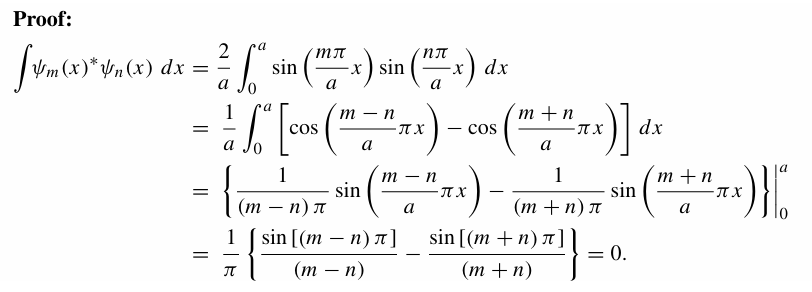
\includegraphics[width = .9\linewidth,trim=0cm 0 0 4mm]{QM_proof1.png}
	\end{figure}

\end{frame}

\begin{frame}{More notes}
	\begin{enumerate}
		\setcounter{enumi}{3}
		\item They are \textbf{complete} i.e. any function can be expressed in terms of linear combinations of $\psi_n(x)$. (This is practically always true but not in general...) $$ f(x) = \sum_{n=1}^{\infty} c_n \psi_n(x)	= \sqrt{\frac 2a } \sum_{n=1}^{\infty} c_n \sin(\frac{n\pi}{a} x)$$ (sometimes called the Dirichlet Theorem). Using Fourier's trick we can get the coefficient $c_n$ to be  $$ c_n = \int \psi_n(x)^* f(x) \dd{x} $$
	\end{enumerate}
\end{frame}

\begin{frame}{Back to the square well}
	The stationary states for the square well are
	\[
		\Psi_n(x,t) = \sqrt{\frac 2a} \sin(\frac{n\pi}{a}x) \exp(-i \frac{n^2\pi^2 \hbar^2}{2ma^2}t)
	\]
	(remember the time factor from eq. \ref{eq:GeneralSol}) and therefore the general solution for the infinite square well is
	\begin{equation}
		\label{eq:sol_sqwell}
		\Psi(x,t) = \sum_{n=1}^{\infty}c_n \sqrt{\frac 2a} \sin(\frac{n\pi}{a}x)e^{-i (n^2\pi^2 \hbar^2/2ma^2)t}
	\end{equation}
	With the $c_n$ to be
	\begin{equation}
		c_n = \sqrt{\frac 2a} \int_{0}^{a} \sin(\frac{n\pi}{a}x) \Psi(x,0) \dd{x}
	\end{equation}

\end{frame}

\subsection{Harmonic Oscillator}
\begin{frame}{The Harmonic Oscillator}
	The potential has the form $$ V(x) = \frac 12 kx^2 = \frac 12 m\omega^2 x^2$$ giving us the following TISE
	$$-\frac{\hbar^2}{2m} \dv[2]{\psi}{x} + \frac 12 m\omega^2x^2 \psi = E \psi$$
	This can be solved in 2 ways : Algebraic (using ladder operators) and Analytic  (power series solution).
	First the Algebraic method
\end{frame}
\begin{frame}{Algebraic method (Ladder operators)}
	We rewrite the TISE in the following form
	\[
		\frac{1}{2m} \qty[\hat{p}^2 + (m\omega x)^2]\psi =E\psi
	\]
	and invoke the ladder operators (I write it here in two equivalent forms Griffiths' and Sakurai's)

	\textbf{Note} $a_+ = a^\dag$ so $a_- = a$ in Sakurai's notation


	\begin{align*}
		\hat{a}_{\pm} = \frac{1}{\sqrt{2\hbar m \omega }} (m\omega x \; \mp i \hat p) &  & \hat{a}_{\pm} = \sqrt{\frac{m\omega}{2\hbar}} \qty(x \mp \frac{i p }{m\omega})
	\end{align*}

\end{frame}

% \include{Questions/P4}
% \include{Questions/P5}
% \include{Questions/P6}


% \frame{Here is what I want to talk about}

\end{document}
